\section{RISC-V Description in SelectionDAG}
\subsection{TableGen Record Declaration}
\begin{frame}{TableGen}
    \begin{itemize}
        \item Domain-specific language used in LLVM backend side to generate CPP header files.
        \item
        Removes redundancy of instruction declaration code
        \item
        Classes are used to convey common information and get inherited to records
        \item
        Declarative instead of Imperative
    \end{itemize}
\end{frame}

\begin{frame}[fragile]{RISC-V TableGen Classes}
Target Independent Instruction Classes
    \begin{itemize}
        \item \textbf{InstructionEncoding}, decoder method, size of instruction
        \item
        \textbf{Instruction}, input and output DAGs
    \end{itemize}
RISC-V Instruction Classes Inherited to declare 'XOR' Instruction
    \begin{itemize}
        \item \textbf{RVInst}, universal bit patterns of RISC-V
        \item
        \textbf{RVInstR}, R type instruction
        \item
        \textbf{ALU\_rr}, features like Commutability declared
    \end{itemize}
\begin{lstlisting}
def XOR  : ALU_rr<0b0000000, 0b100, "xor", /*Commutable*/1>,
           Sched<[WriteIALU, ReadIALU, ReadIALU]>;
\end{lstlisting}
\end{frame}


\subsection{TableGen Pattern Matching}
\begin{frame}[fragile]{TableGen Patterns}
RISC-V TableGen classes can be used to declare any instruction in a more structured way.
\par
The DAG pattern of the instruction can be declared in a Pattern declaration of TableGen. For the NAXOR (NOT AND XOR) instruction, it is: LLVM IR assembly instructions and intrinsic functions are combined in DAG structure.

\begin{lstlisting}
def : Pat< (xor (and (not GPR:$src1), GPR:$src2), GPR:$src3),
(NAXOR GPR:$src1, GPR:$src2, GPR:$src3)>;
\end{lstlisting}
\end{frame}

        
        

\begin{frame}[fragile]{TableGen Patterns}
\begin{lstlisting}
let hasSideEffects = 0, mayLoad = 0, mayStore = 0 in
class ALU_rrr<bits<2> funct2, bits<3> funct3, string opcodestr,
             bit Commutable = 0>
    : RVInstR4<funct2, funct3, OPC_OP, (outs GPR:$rd), (ins GPR:$rs1, GPR:$rs2, GPR:$rs3),
              opcodestr, "$rd, $rs1, $rs2 ,$rs3"> {
  let isCommutable = Commutable;
}
\end{lstlisting}
A custom class of instruction named ALU\_rrr is created. MLA instruction requires three source registers and is defined to be ALU type. 
\end{frame}


        
\begin{frame}[fragile]{TableGen Patterns}
\begin{lstlisting}
def NAXOR     : ALU_rrr<0b11, 0b100, "naxor">,
Sched<[WriteIMul, ReadIMul, ReadIMul]>;
\end{lstlisting}
MLA instruction is defined and ALU\_rrr instruction type is used. funct2,funct3, opcode string and schedules are sufficient to have the full definition of the instruction thanks to the custom ALU\_rrr class.
\end{frame}



\begin{frame}[fragile]{TableGen Patterns}
\begin{figure}
    \centering
    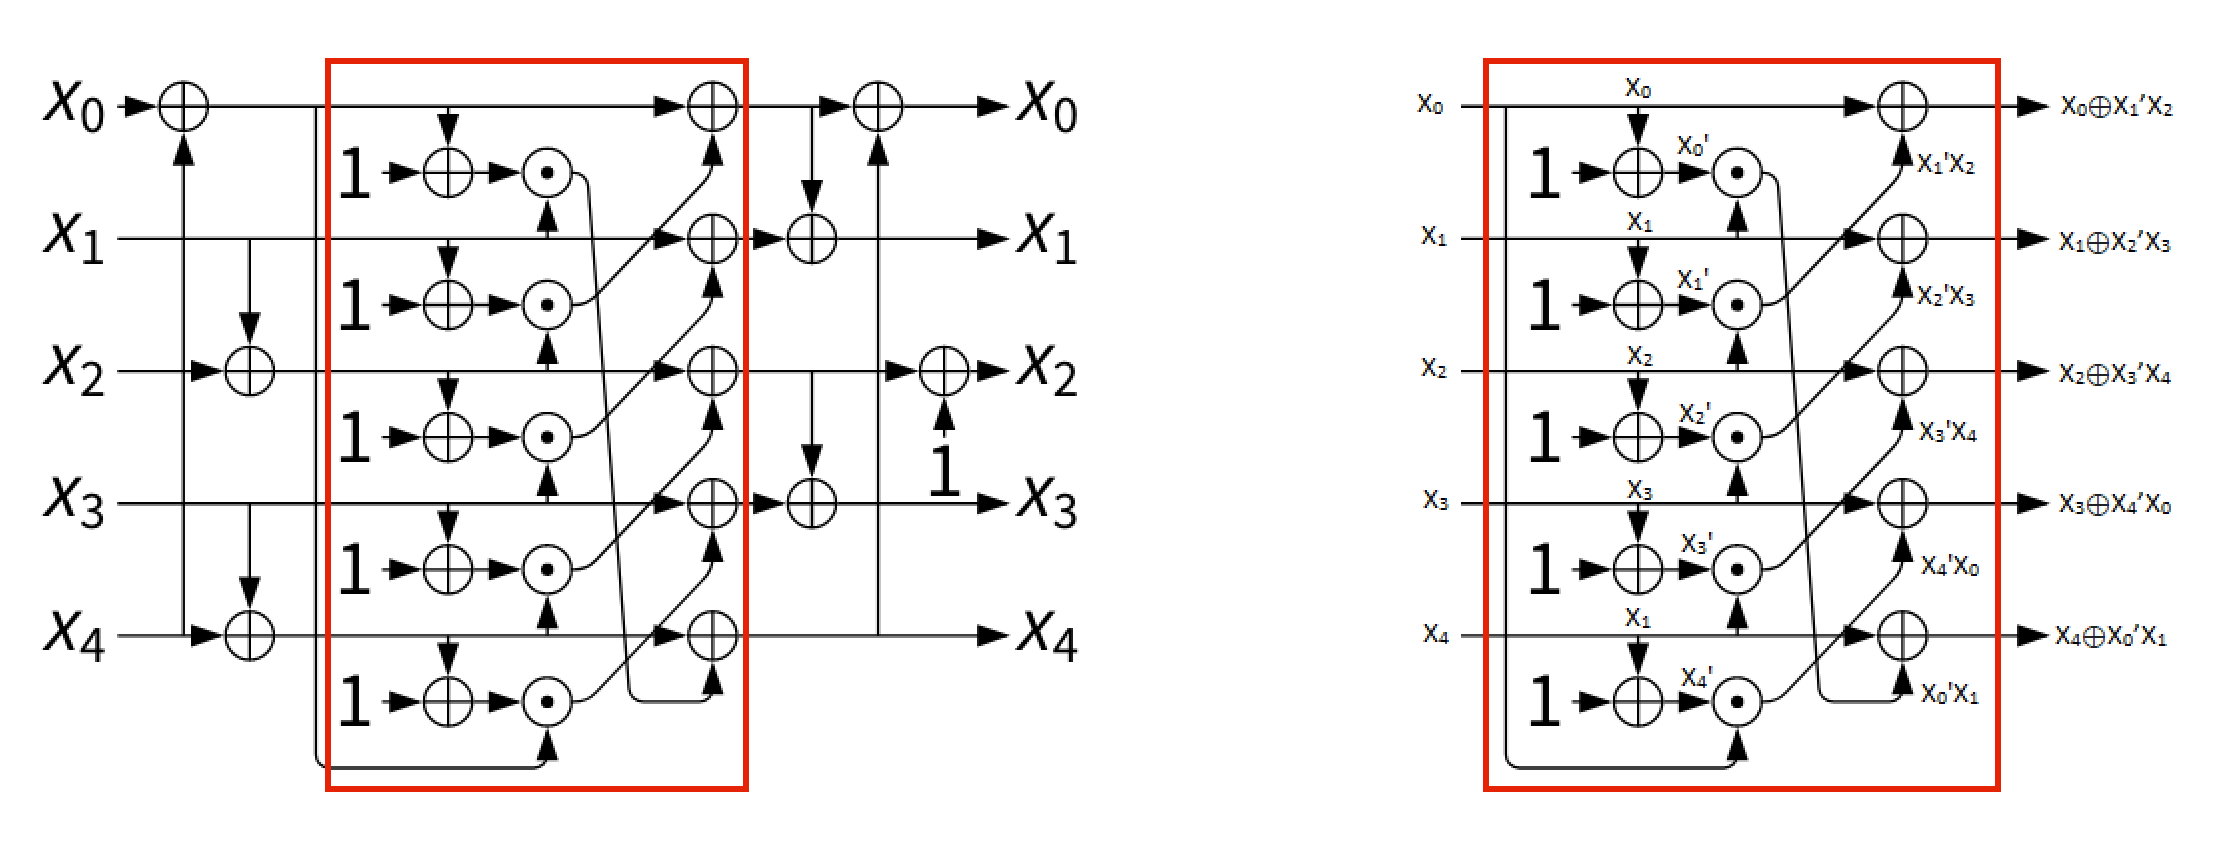
\includegraphics[scale=0.3]{sbox_naxor_pattern.png}
    \caption{NAXOR patterns in s-box algorithm}
    \label{fig:sbox_naxor_pattern}
\end{figure}
This pattern is repeated 5 times as emphasized in Figure \ref{fig:sbox_naxor_pattern}. NAXOR instruction reduces 15 instructions into 5 instructions.
\end{frame}



\begin{frame}[fragile]{TableGen Patterns}
\begin{figure}
    \centering
    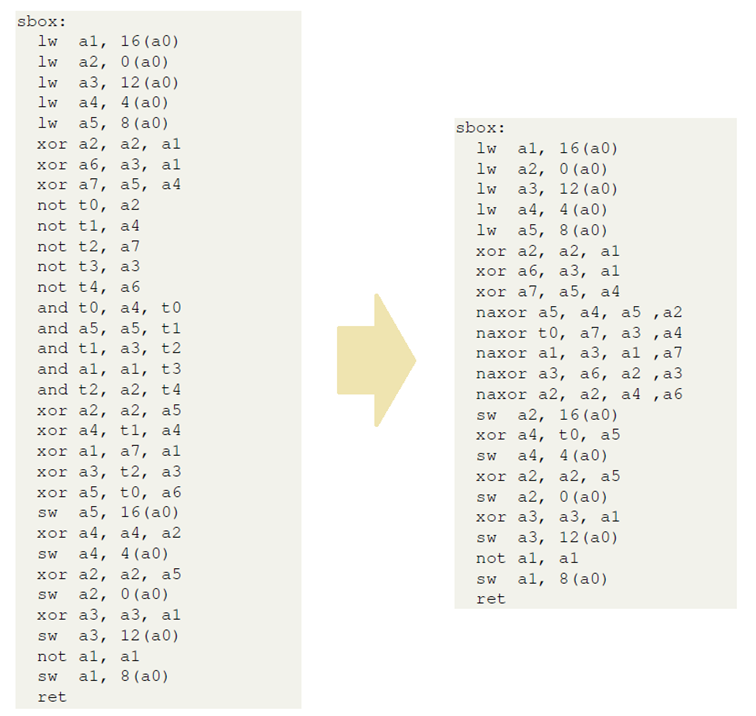
\includegraphics[scale=0.3]{naxor_instruction.png}
    \caption{NAXOR instruction's effect on S-BOX assembly code}
    \label{fig:sbox_instruction}
\end{figure}
The S-box algorithm includes a certain pattern that is used repeatedly.
NOT-AND-XOR pattern is used five times in an s-box cycle. This pattern is lowered
into one instruction using TableGen. After matching this pattern 15 rows of the
assembly file are reduced to one single instruction.
\end{frame}
